\chapter{نحوه‌ی کار و ارزیابی}\label{chapter4}

\section{نحوه‌ی کار با بستر بدون سرور اینترنت اشیاء}

برای آشنایی با نحوه‌ی کار کردن با بستر بدون سرور اینترنت اشیاء به پیاده‌سازی یک برنامه‌ی کاربردی تست با استفاده از امکانات موجود این بستر می‌پردازیم. این برنامه‌‌ی کاربردی در دو قسمت سرویس دهنده و سرویس گیرنده پیاده‌سازی شده است. اصلی‌ترین بخش یک برنامه‌ی کابردی، منطق آن برنامه است که سمت سرور پیاده‌سازی شده و اجرا می‌شود. در این بستر بدون سرور منطق برنامه باید با استفاده از تابع‌ها به عنوان \lr{action} های بستر \lr{OpenWhisk} پیاده‌سازی شود. بنابراین منطق کلی برنامه ابتدا باید تا سطح تابع‌های مجزا بخش شود و سپس نحوه‌ی اتصال این تابع‌ها برای ایجاد آن بخش از منطق برنامه تعیین گردد. برای پیاده‌سازی بخش‌های پیچیده‌ی منطق برنامه، می‌توان از امکانات بستر \lr{OpenWhisk} مانند اتصال تابع‌ها به یکدیگر یا ایجاد \lr{rule} کمک گرفت. در انتها برای ارائه‌ی سرویس به سرویس گیرنده، تابع‌های مورد نظر به عنوان  \lr{REST API} تعریف شده و سرویس گیرنده می‌تواند با ارسال درخواست‌های \lr{HTTP}، به سرویس مورد نیازش دسترسی داشته باشد. شکل \ref{tok-work-flow} مراحل کار با این بستر را نشان می‌دهد.

\begin{figure}[!h]
	\centering
	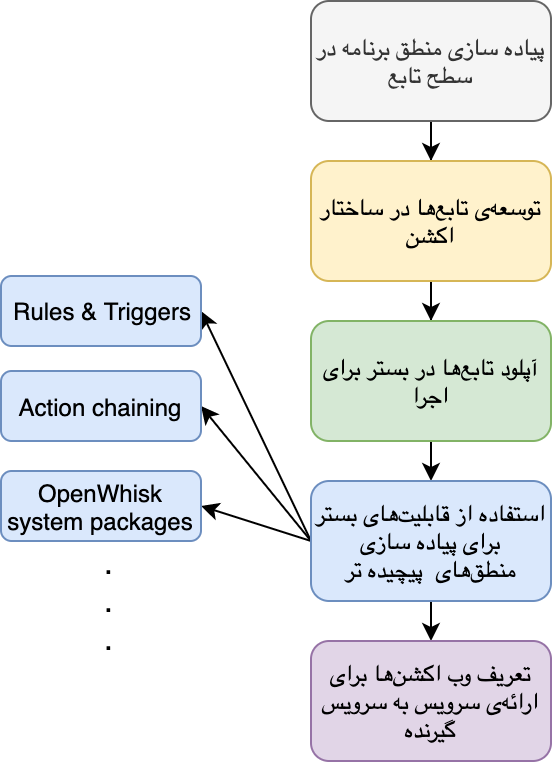
\includegraphics[height=9cm]{images/tok-work-flow}
	\caption{مراحل کار با بستر بدون سرور اینترنت اشیاء}
	\label{tok-work-flow}
\end{figure}

برنامه‌ی کاربردی تست در نظر گرفته شده، یک برنامه‌ی کابردی تلفن همراه است که دستگاه‌های متصل به بستر را نمایش می‌دهد و با انتخاب هر دستگاه، داده‌های ارسالی توسط آن دستگاه به صورت بلادرنگ قابل مشاهده خواهد بود.

\subsection{سرویس دهنده}

برای نمونه نحوه‌ی پیاده‌سازی یکی از \lr{action} های این برنامه به نام \lr{getTelemetryKeys} را بررسی می‌کنیم(شکل \ref{action-file}). این \lr{action} با گرفتن ‌\lr{token} دستگاه، با اتصال به پایگاه داده‌ی سری زمانی، کلیدهای داده‌هایی که آن دستگاه ارسال کرده است را پیدا کرده و برمی‌گرداند. \lr{token} هر دستگاه یک \lr{string} است که مخصوص همان دستگاه است و با استفاده از آن می‌توان داده‌های ذخیره شده در پایگاه داده سری زمانی را برای هر دستگاه استخراج کرد. برای استخراج این داده‌ها از پایگاه داده باید درخواست موردنظر با زبان درخواست \lr{InfluxDB} نوشته شود و سپس با یک درخواست \lr{HTTP} به سرویس دهنده‌ی \lr{HTTP} پایگاه داده ارسال شود. آدرس پایگاه داده درون خوشه‌ی کوبرنتیز، برابر نام سرویس \lr{ClusterIP} آن پایگاه داده است و \lr{port} آن نیز باید مشخص شود. بقیه‌ی تنظیمات این درخواست \lr{HTTP} باید مطابق با \lr{API} پایگاه داده‌ی \lr{InfluxDB} انجام شود. پایگاه داده نتیجه‌ی درخواست را در جواب برمی‌گرداند. در انتها باید این نتیجه توسط \lr{action} تعریف شده برگردانده شود. این امر به دلیل این که درخواست \lr{HTTP} ناهمگام است به سادگی امکان پذیر نیست، زیرا \lr{action} باید منتظر جواب درخواست \lr{HTTP} بماند و سپس نتیجه را برگرداند. بنابراین از ساختار \lr{promise} زبان \lr{JavaScript} استفاده شده است. ساختار \lr{promise} این امکان را می‌دهد که \lr{action} خروجی خود را با تأخیر و به صورت ناهمگام برگرداند. 

\begin{figure}[!h]
	\centering
	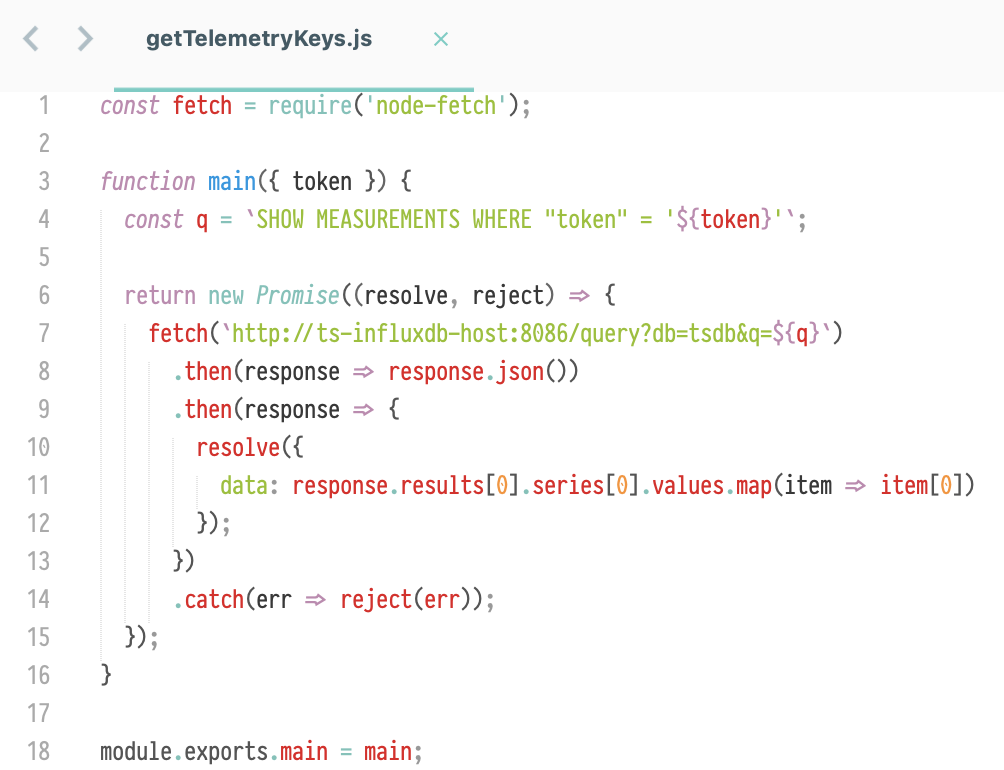
\includegraphics[height=10cm]{images/action-file}
	\caption{تابع نوشته شده برای \lr{getTelemetryKeys action}}
	\label{action-file}
\end{figure}

حال پس از پیاده‌سازی این \lr{action}، نوبت به اجرا می‌رسد. برای اجرا ابتدا باید کتابخانه‌های مورد نیاز این \lr{action} نصب شوند. سپس برای ارزیابی، این تابع با استفاده از توابع دیگر که برای تست نوشته شده‌اند به صورت محلی اجرا می‌شود. در صورت موفقیت آمیز بودن ارزیابی، فایل تابع به همراه کتابخانه‌ها، \lr{zip} شده و با استفاده از اجرای یک دستور در محیط \lr{CLI} مربوط به \lr{OpenWhisk} به نام \lr{wsk}، در بستر آپلود می‌شود. این دستور مورد استفاده در شکل \ref{wsk-cli} نشان داده شده است.

\begin{figure}[!h]
	\centering
	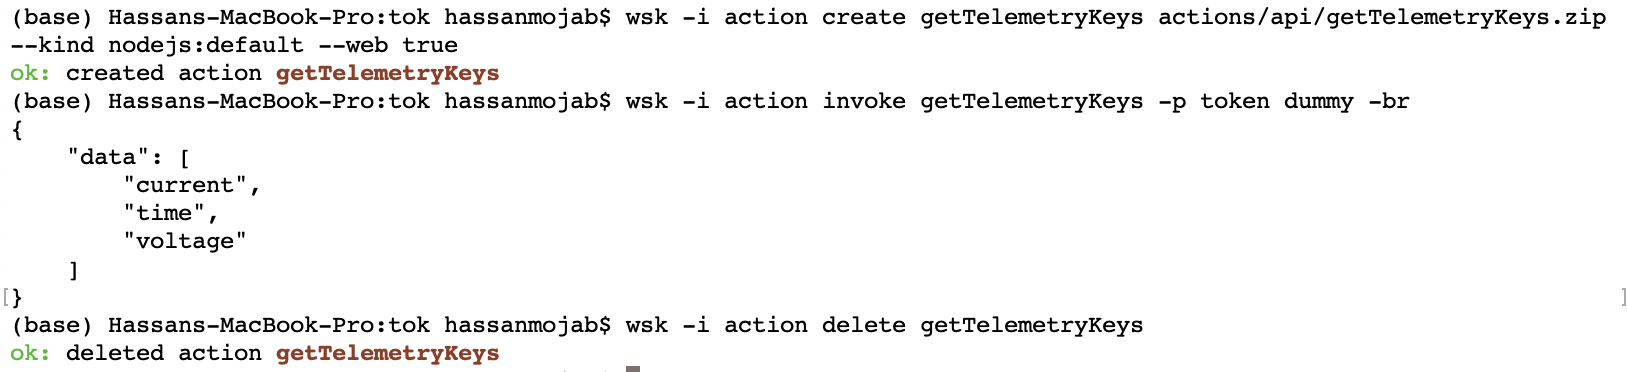
\includegraphics[height=3.7cm]{images/wsk-cli}
	\caption{آپلود، اجرا و حذف \lr{action} با استفاده از دستور \lr{wsk}}
	\label{wsk-cli}
\end{figure}

\subsection{سرویس گیرنده}

سرویس گیرنده‌ی طراحی شده برای این برنامه‌ی تست، یک برنامه‌ی کاربردی تلفن همراه است که با استفاده از فریم وورک \lr{React Native} پیاده‌سازی شده است. این برنامه‌ی کابردی از \lr{REST API} های تعریف شده توسط سرویس دهنده استفاده می‌کند و دستگاه‌ها و داده‌های مربوط به آن‌ها را نمایش می‌دهد. این برنامه یک واسط کاربری گرافیکی\LTRfootnote{GUI} تلقی شده و با مصورسازی داده‌ها برای سهولت درک کارکرد این بستر طراحی شده است. در ادامه تصویری از این برنامه نمایش داده شده است (شکل \ref{app}).

\begin{figure}[!h]
	\centering
	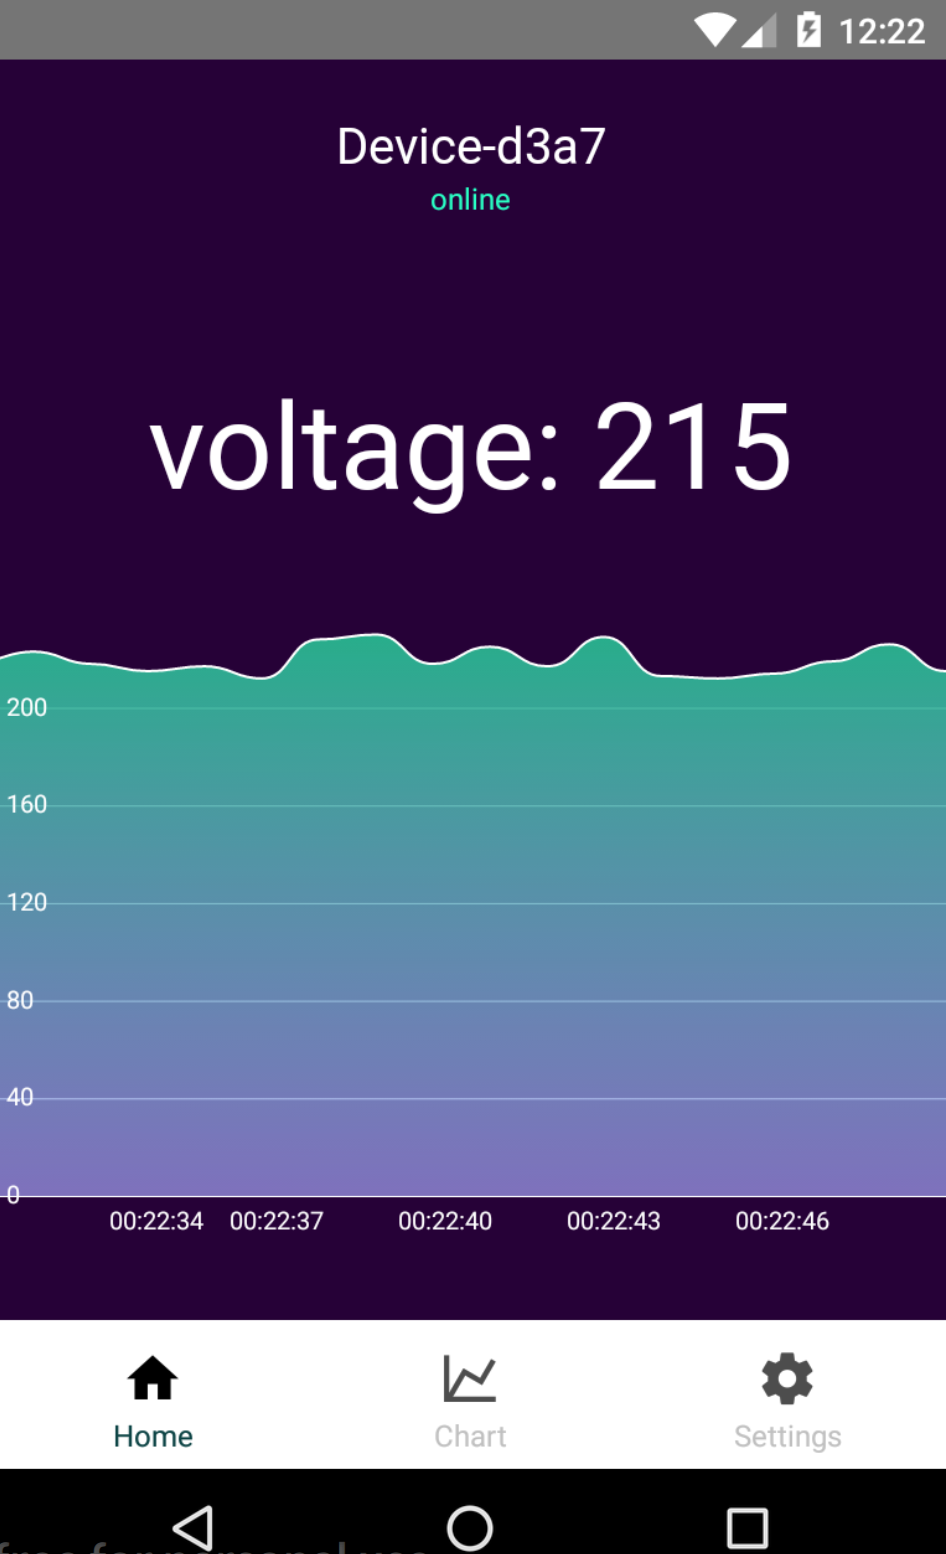
\includegraphics[height=10cm]{images/app}
	\caption{برنامه کاربردی تلفن همراه طراحی شده}
	\label{app}
\end{figure}

\newpage

\section{ارزیابی بستر بدون سرور اینترنت اشیاء}

برای اطمینان از صحت کارکرد بستر بدون سرور اینترنت اشیاء، این بستر در بخش‌های مختلف ارزیابی شده و نتایج آن مورد بررسی قرار گرفت. برای ارزیابی بخش سمت دستگاه‌های اینترنت اشیاء باید شبکه‌ای شبیه سازی شده از دستگاه‌های اینترنت اشیاء به بستر متصل شود. برای شبیه سازی دستگاه اینترنت اشیاء، یک اسکریپت نوشته شده است که با اتصال به \lr{MQTT message broker} از طریق شبکه‌ی اینترنت، هر ثانیه یک پیام \lr{MQTT}، شامل \lr{token} آن دستگاه و داده‌های تولید شده به صورت تصادفی را به بستر ارسال کند. با اجرای چندین نمونه از این اسکریپت با \lr{token} های مختلف می‌توان شبکه‌ی دستگاه‌های اینترنت اشیاء را شبیه‌سازی کرد. پس از اتصال این شبکه، زمان ارسال پیام توسط دستگاه به عنوان یک داده ارسال شده تا با زمان ذخیره در پایگاه داده مقایسه گردد. اختلاف این دو زمان به طور میانگین برابر با ۳۰۰ میلی ثانیه به دست آمد که با شلوغ شدن شبکه تا ۱۰۰ دستگاه، به ۳ ثانیه افزایش یافت. این زمان برابر است با مجموع تأخیر صف \lr{MQTT message broker}، زمان پردازش \lr{Controller}، تأخیر صف \lr{Kafka} و در نهایت زمان اجرای تابع و ذخیره کردن داده در پایگاه داده.

